\chapter{3D打印建模}
\label{cha:Model}

\section{Model v1}

测试用3轮底盘需要考虑到电机和定位模块的配合。

定位模块外形为 $\phi$ 11.2 X 25.1mm,至少需要留12mm直径的圆柱形空间,头部距离地面不得超过2mm。定位模块外形尺寸如图~\ref{fig:Camera-Dimension}。

\begin{figure}[htbp]
    \centering
    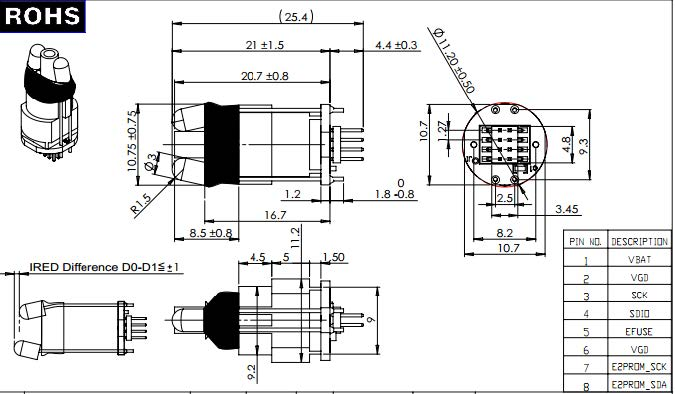
\includegraphics[width=\columnwidth]{SONIX_OID_SNM9S500C3000A_Specification_V1-Dimension.jpg}
    \caption{定位模块外形尺寸}
    \label{fig:Camera-Dimension}
\end{figure}

定位模块配套母排离PCB高度为4.3mm,所以Camera下端居PCB底面约为27mm,根据经验需要预留7-10mm的离地距离,所以按照35mm预留,小于轮子直径38mm,考虑可以加一个延长针脚座使用,所以PCB离地设计为50mm。


底盘装配图如图~\ref{fig:Assembled-Test-Datasheet}。

\begin{figure}[htbp]
    \centering
    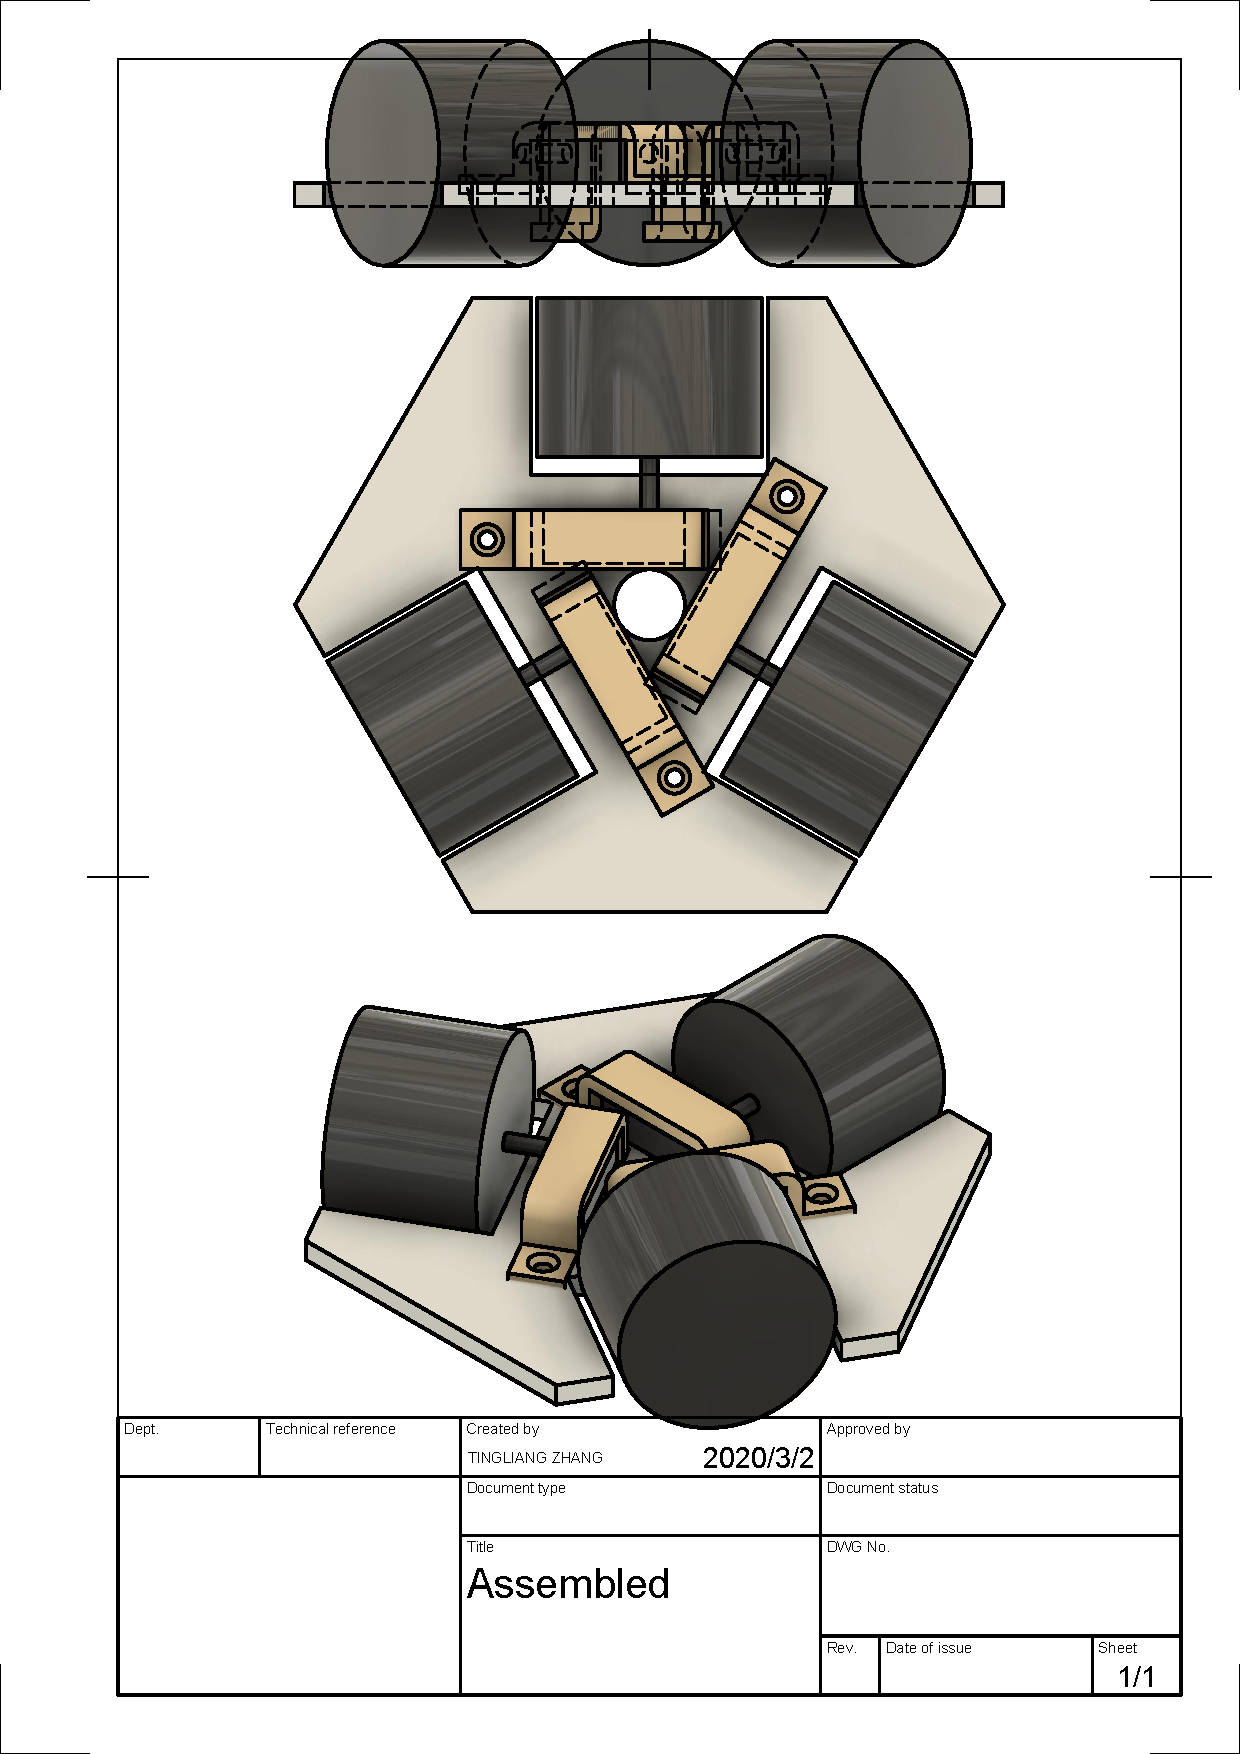
\includegraphics[width=\columnwidth]{Assembled-v1.pdf}
    \caption{测试用底盘装配图}
    \label{fig:Assembled-Test-Datasheet}
\end{figure}

测试用底盘渲染图如图~\ref{fig:Assembled-Test-Render}。

\begin{figure}[htbp]
    \centering
    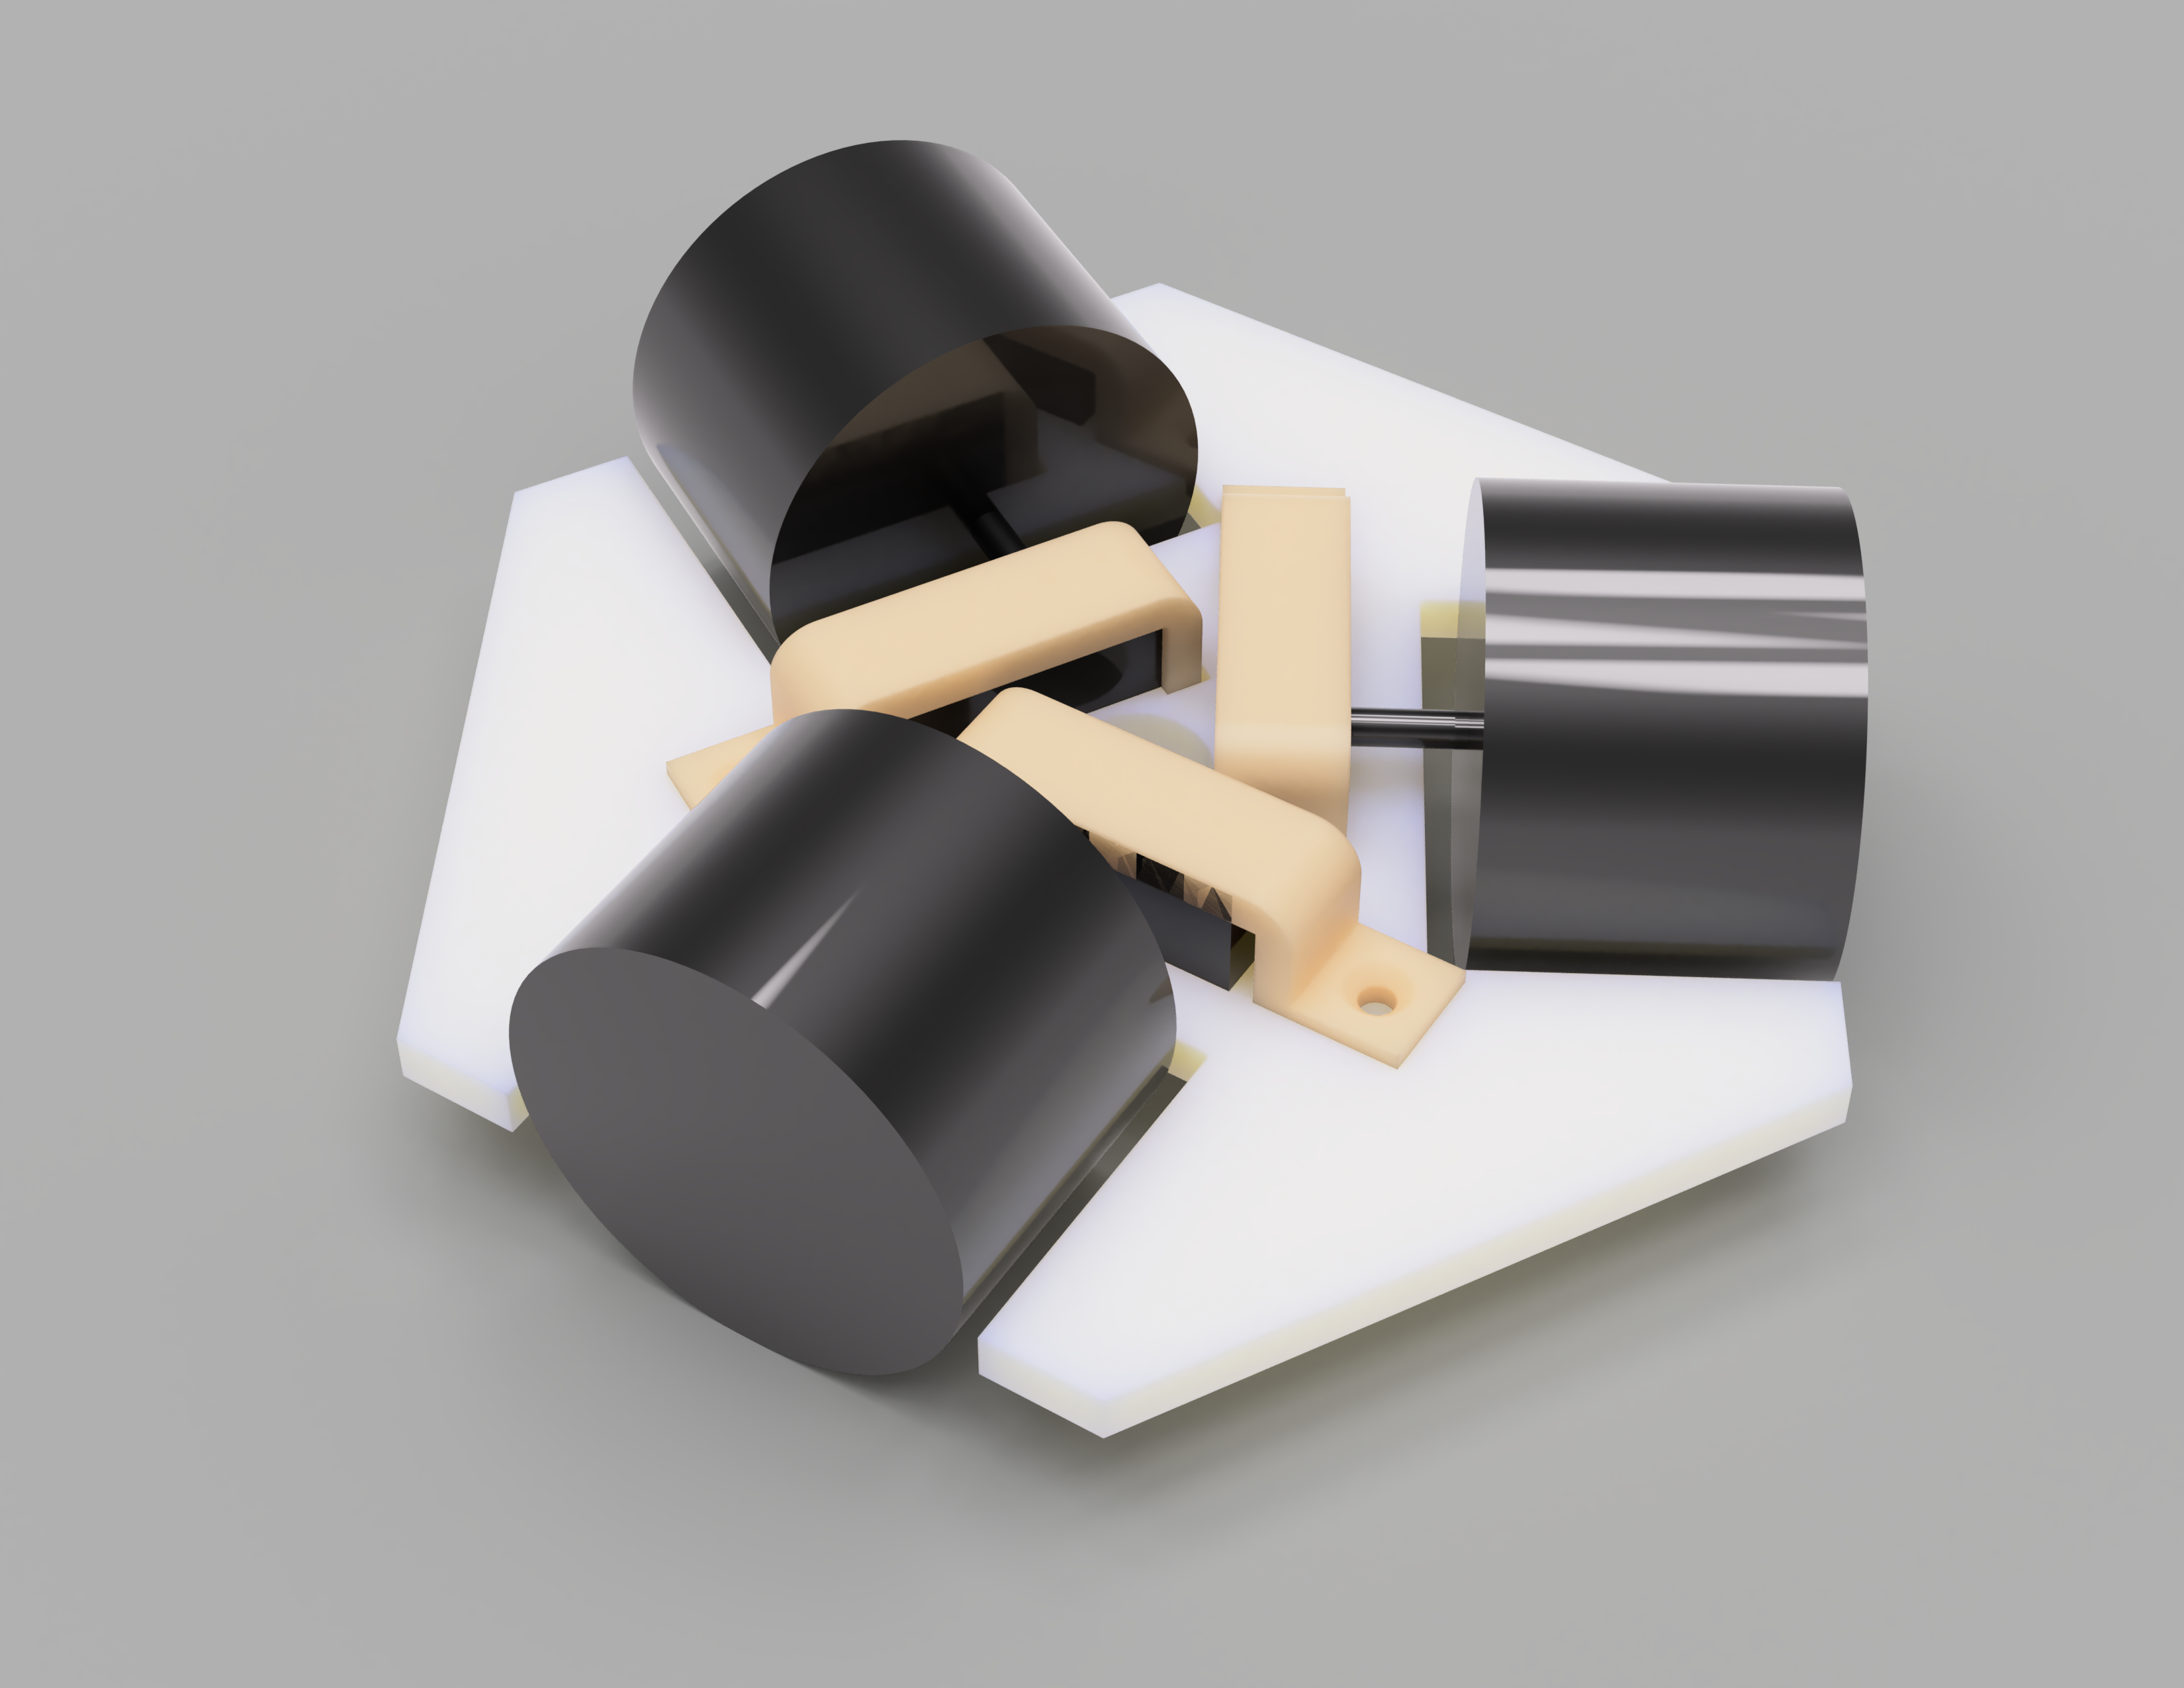
\includegraphics[width=\columnwidth]{Assembled_2020-Mar-02.png}
    \caption{测试用底盘渲染图}
    \label{fig:Assembled-Test-Render}
\end{figure}

其中,电机固定件使用的是一颗沉头M3*10的不锈钢螺栓。固定件上留出大径5.3mm小径3mm的沉头螺丝孔,底板上则留一个直径5.9mm圆内接正六边形深度为2.5mm的六角螺母固定孔,以便不用鸭嘴钳拧螺丝,当然也有3mm的圆孔。如图~\ref{fig:BottomTest-v1-Datasheet}和图~\ref{fig:StepperMount-v1-Datasheet}。

\begin{figure}[htbp]
    \centering
    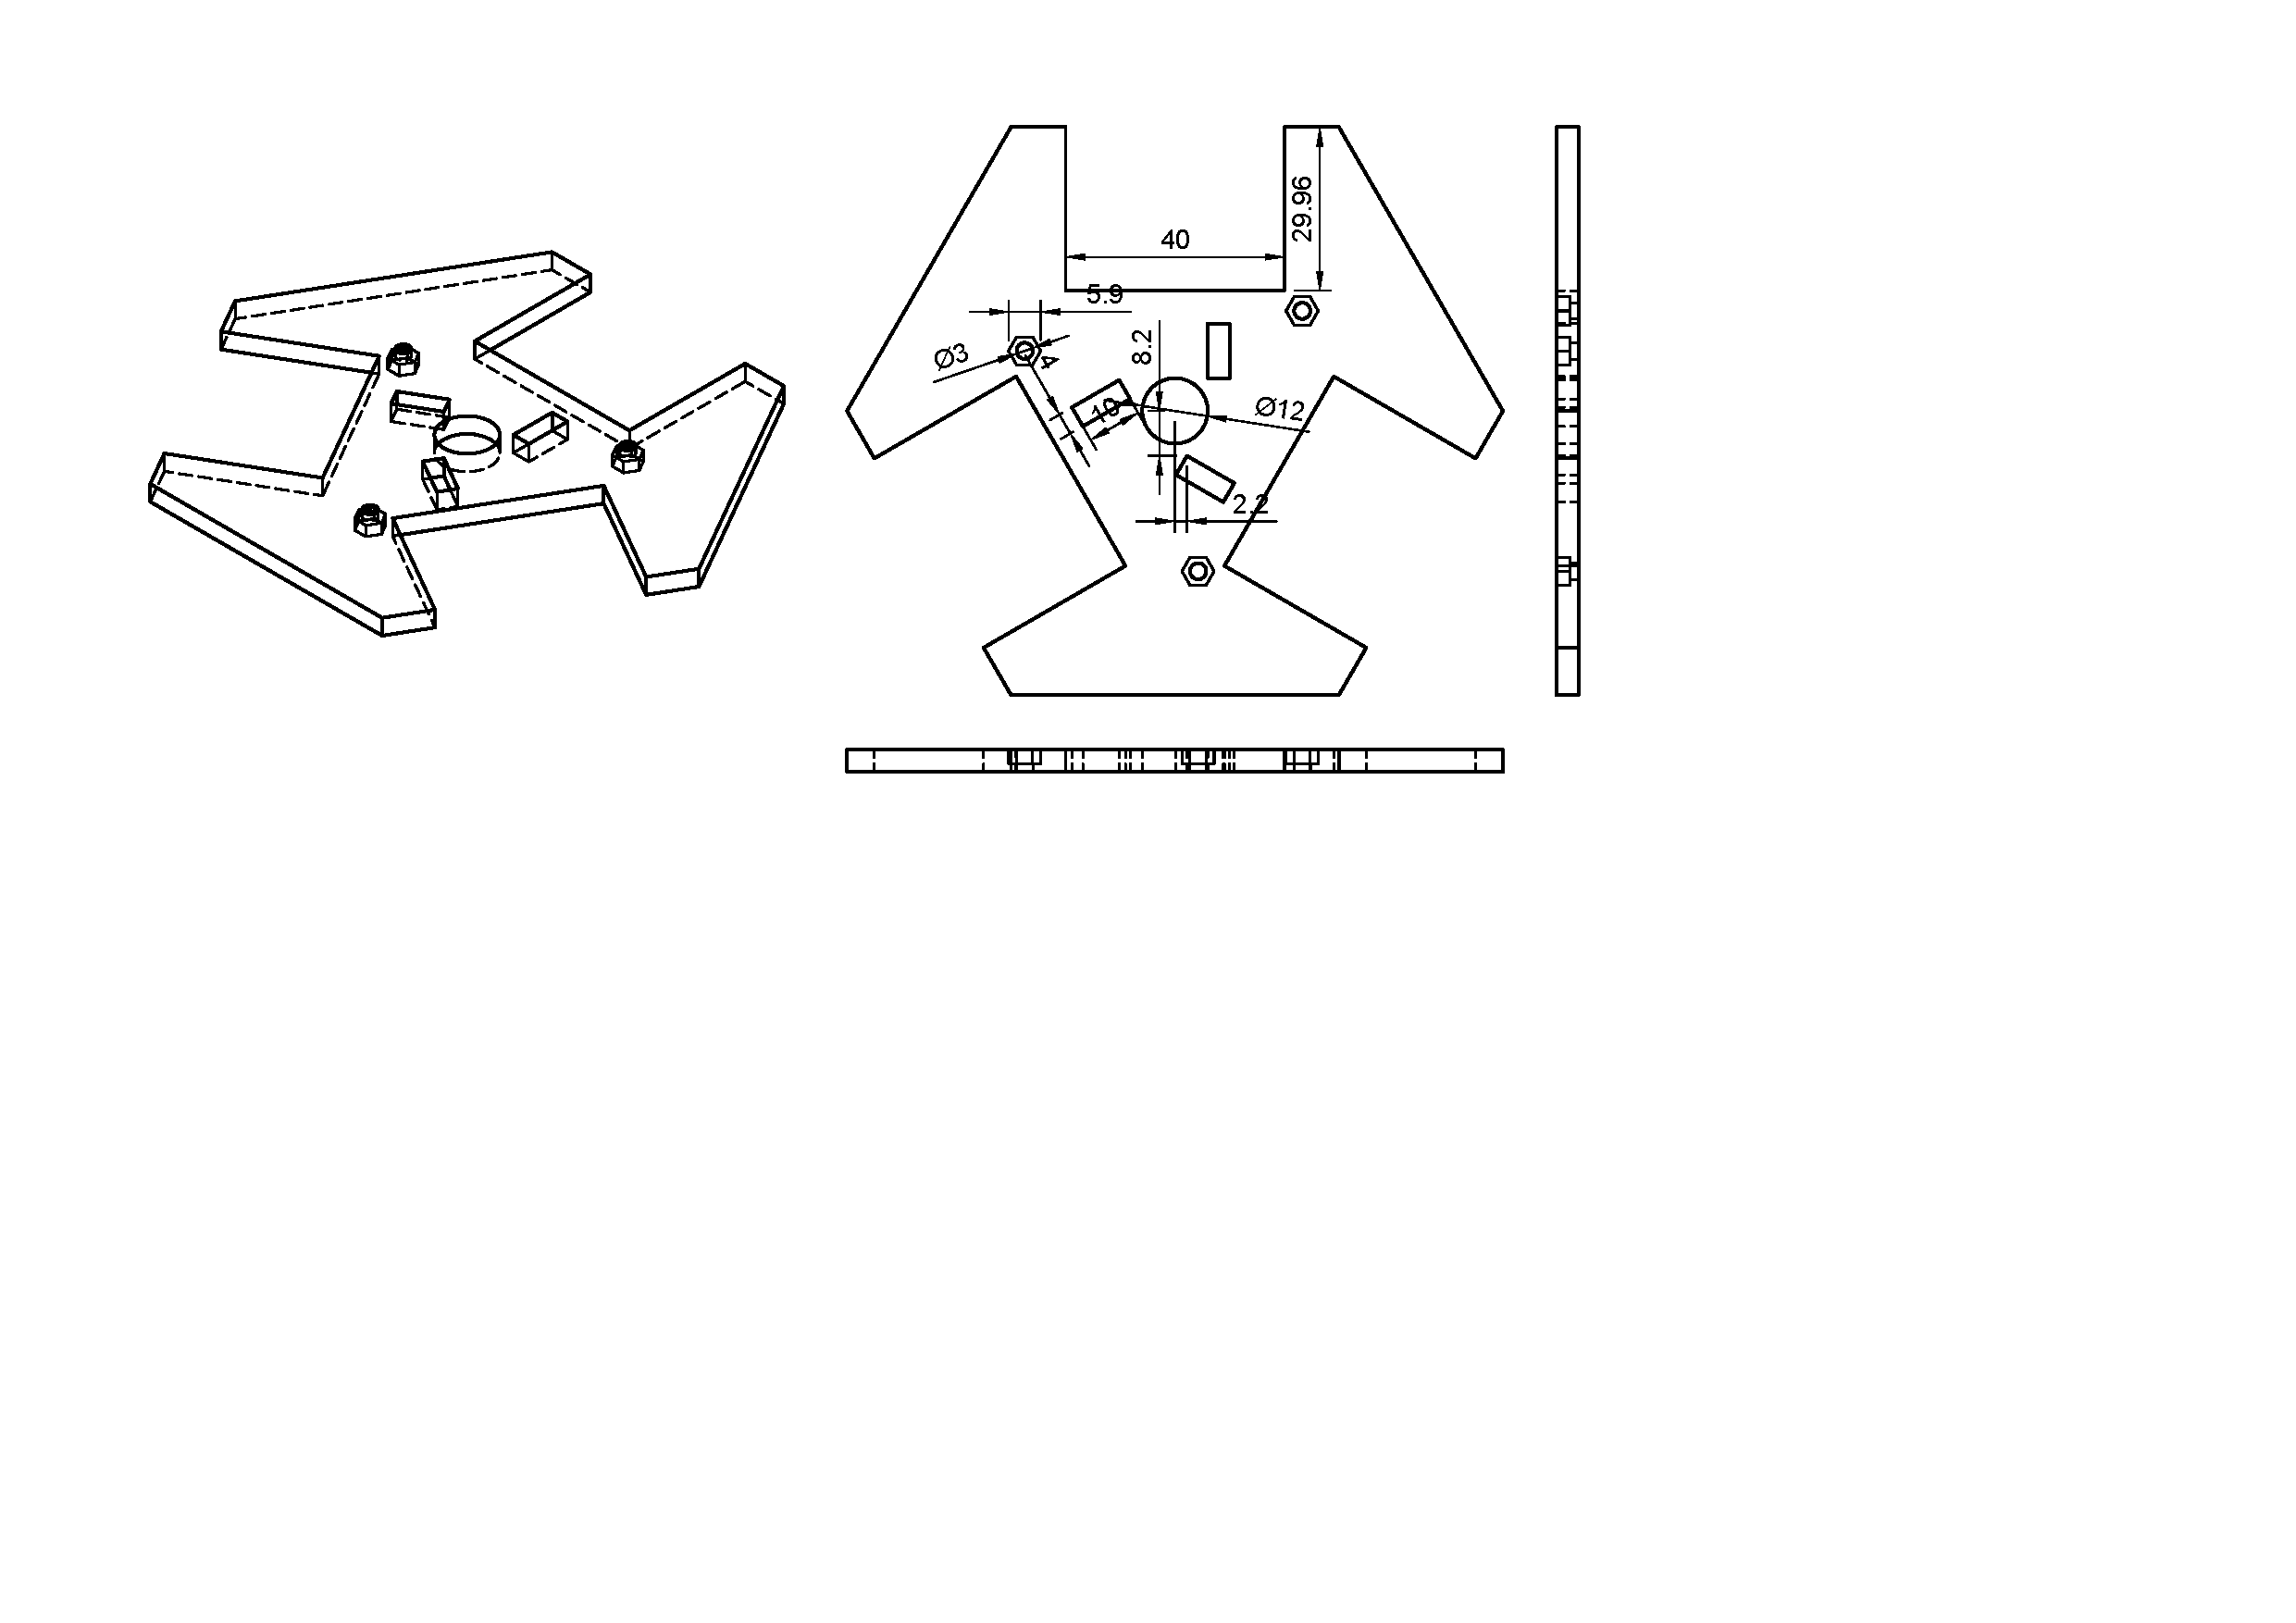
\includegraphics[width=\columnwidth]{BottomTest-v1.pdf}
    \caption{测试用底盘图纸}
    \label{fig:BottomTest-v1-Datasheet}
\end{figure}

由于两电机之间间隙(矩形可延展4.39mm)不足以放下一个M3螺丝,所以采用了一边卡扣的形式来固定。

\begin{figure}[htbp]
    \centering
    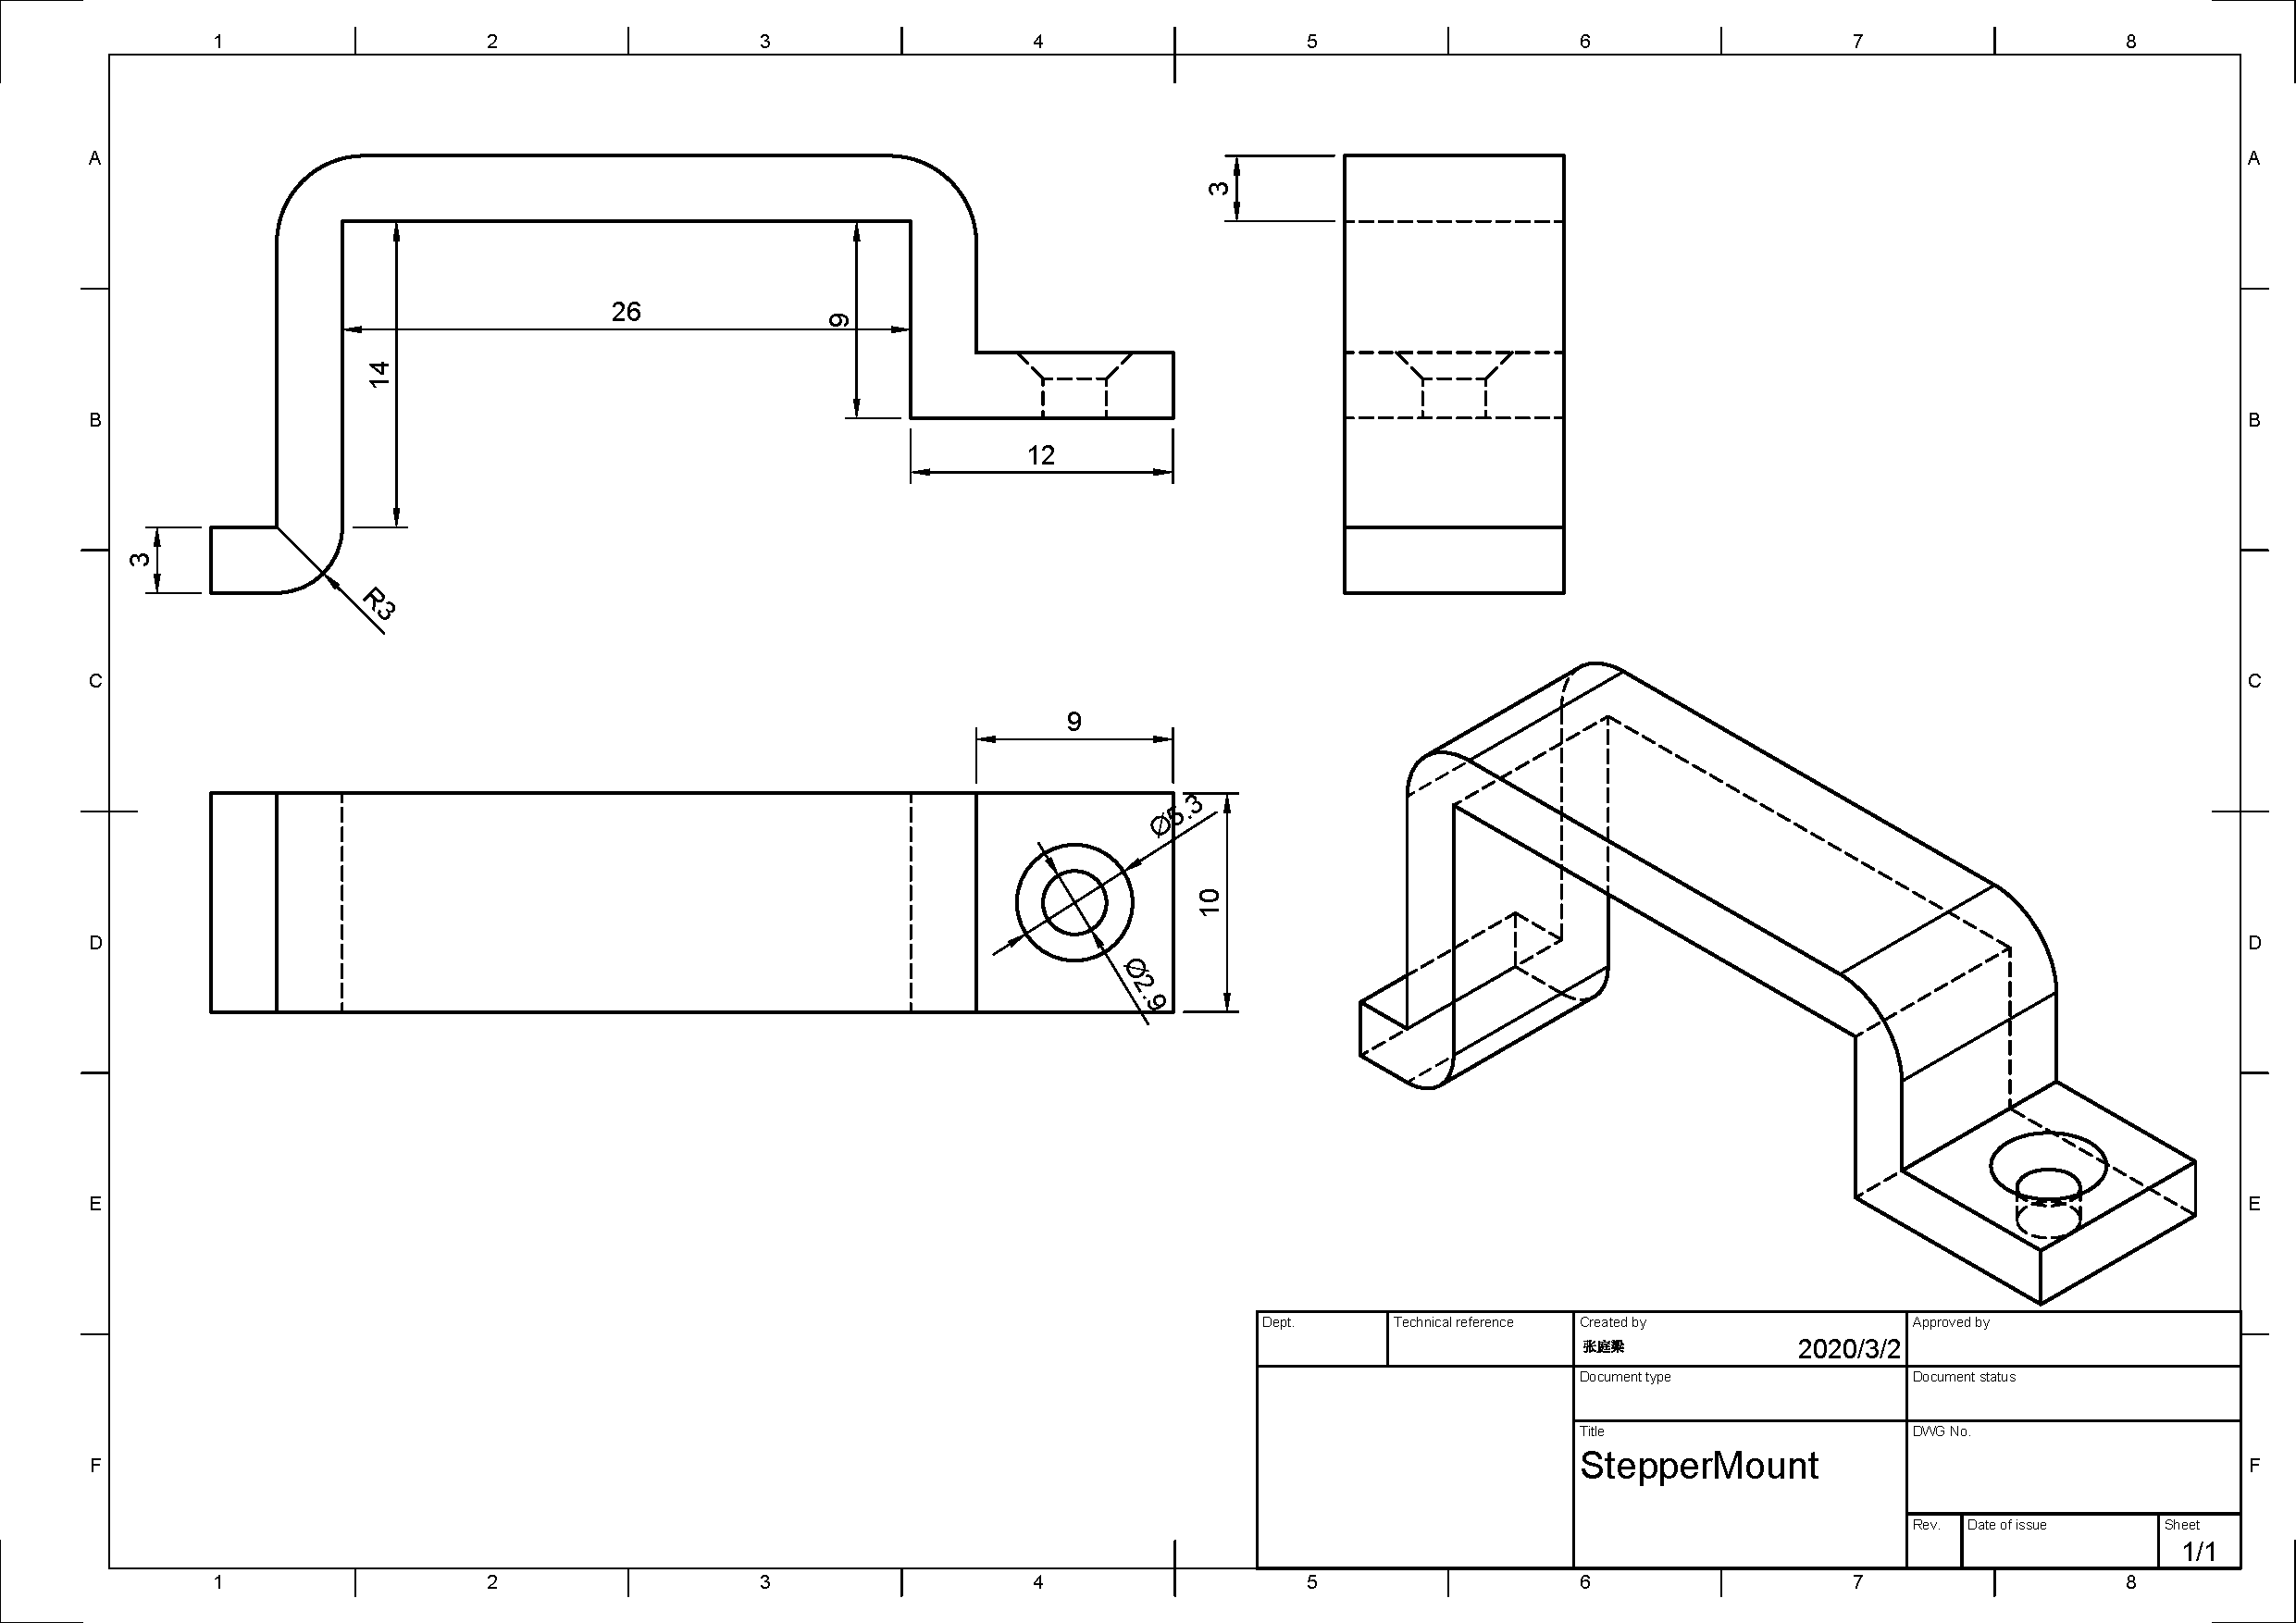
\includegraphics[width=\columnwidth]{StepperMount-v1.pdf}
    \caption{步进电机固定座图纸}
    \label{fig:StepperMount-v1-Datasheet}
\end{figure}

其中步进和轮子画为一个零件,作确定装配体尺寸用,如图~\ref{fig:StepperAndWheel-v0-Datasheet}。

\begin{figure}[htbp]
    \centering
    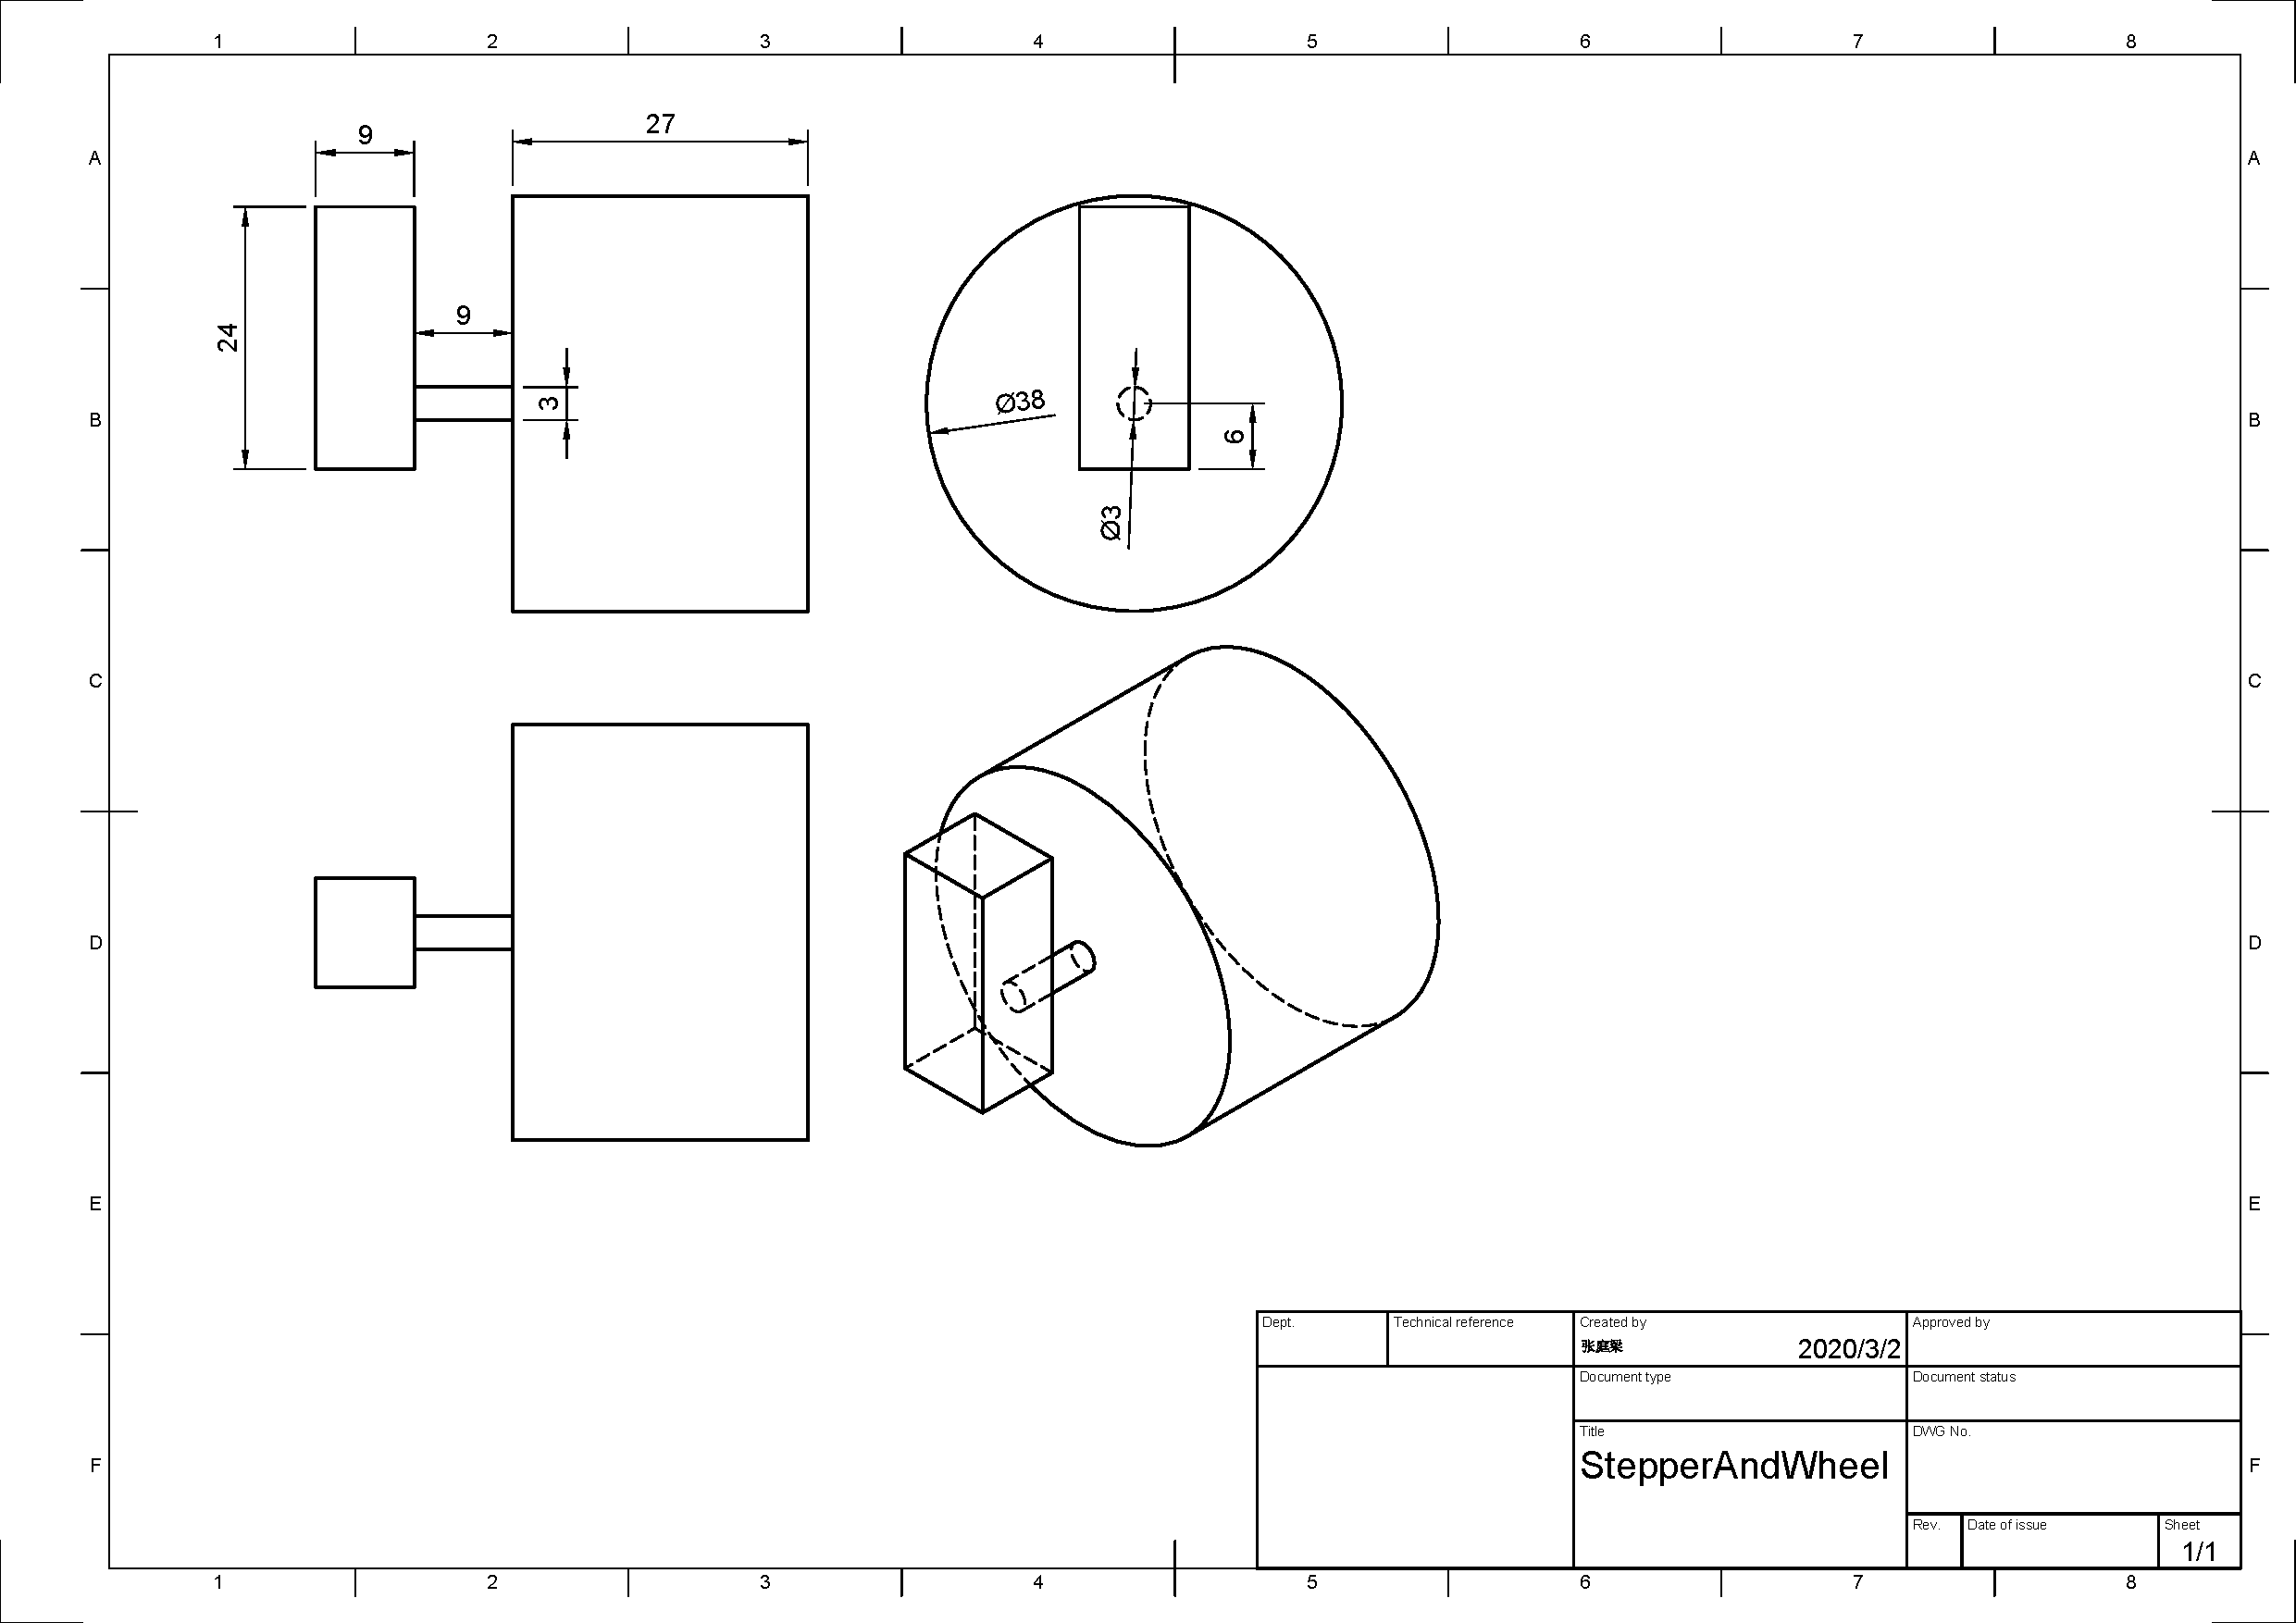
\includegraphics[width=\columnwidth]{StepperAndWheel-v0.pdf}
    \caption{步进和轮子图纸}
    \label{fig:StepperAndWheel-v0-Datasheet}
\end{figure}


电机固定加凹槽,固定一下前后位置。

PCB放置到凹槽里面,固定水平位置


\section{Model v2}

电机固定一颗螺丝固定相邻两个电机,重叠边沿打孔。

采用暴力热熔胶固定的方式,一个长方形固定位,上沿和轮侧面用一根PLA材料热熔胶固定,如图~\ref{fig:Bottomv1}。

\begin{figure}[htbp]
    \centering
    \includegraphics[width=\columnwidth]{Bottomv1.jpg}
    \caption{手掌上的测试底盘}
    \label{fig:Bottomv1}
\end{figure}

图纸如图~\ref{fig:Bottom2v1}。

\begin{figure}[htbp]
    \centering
    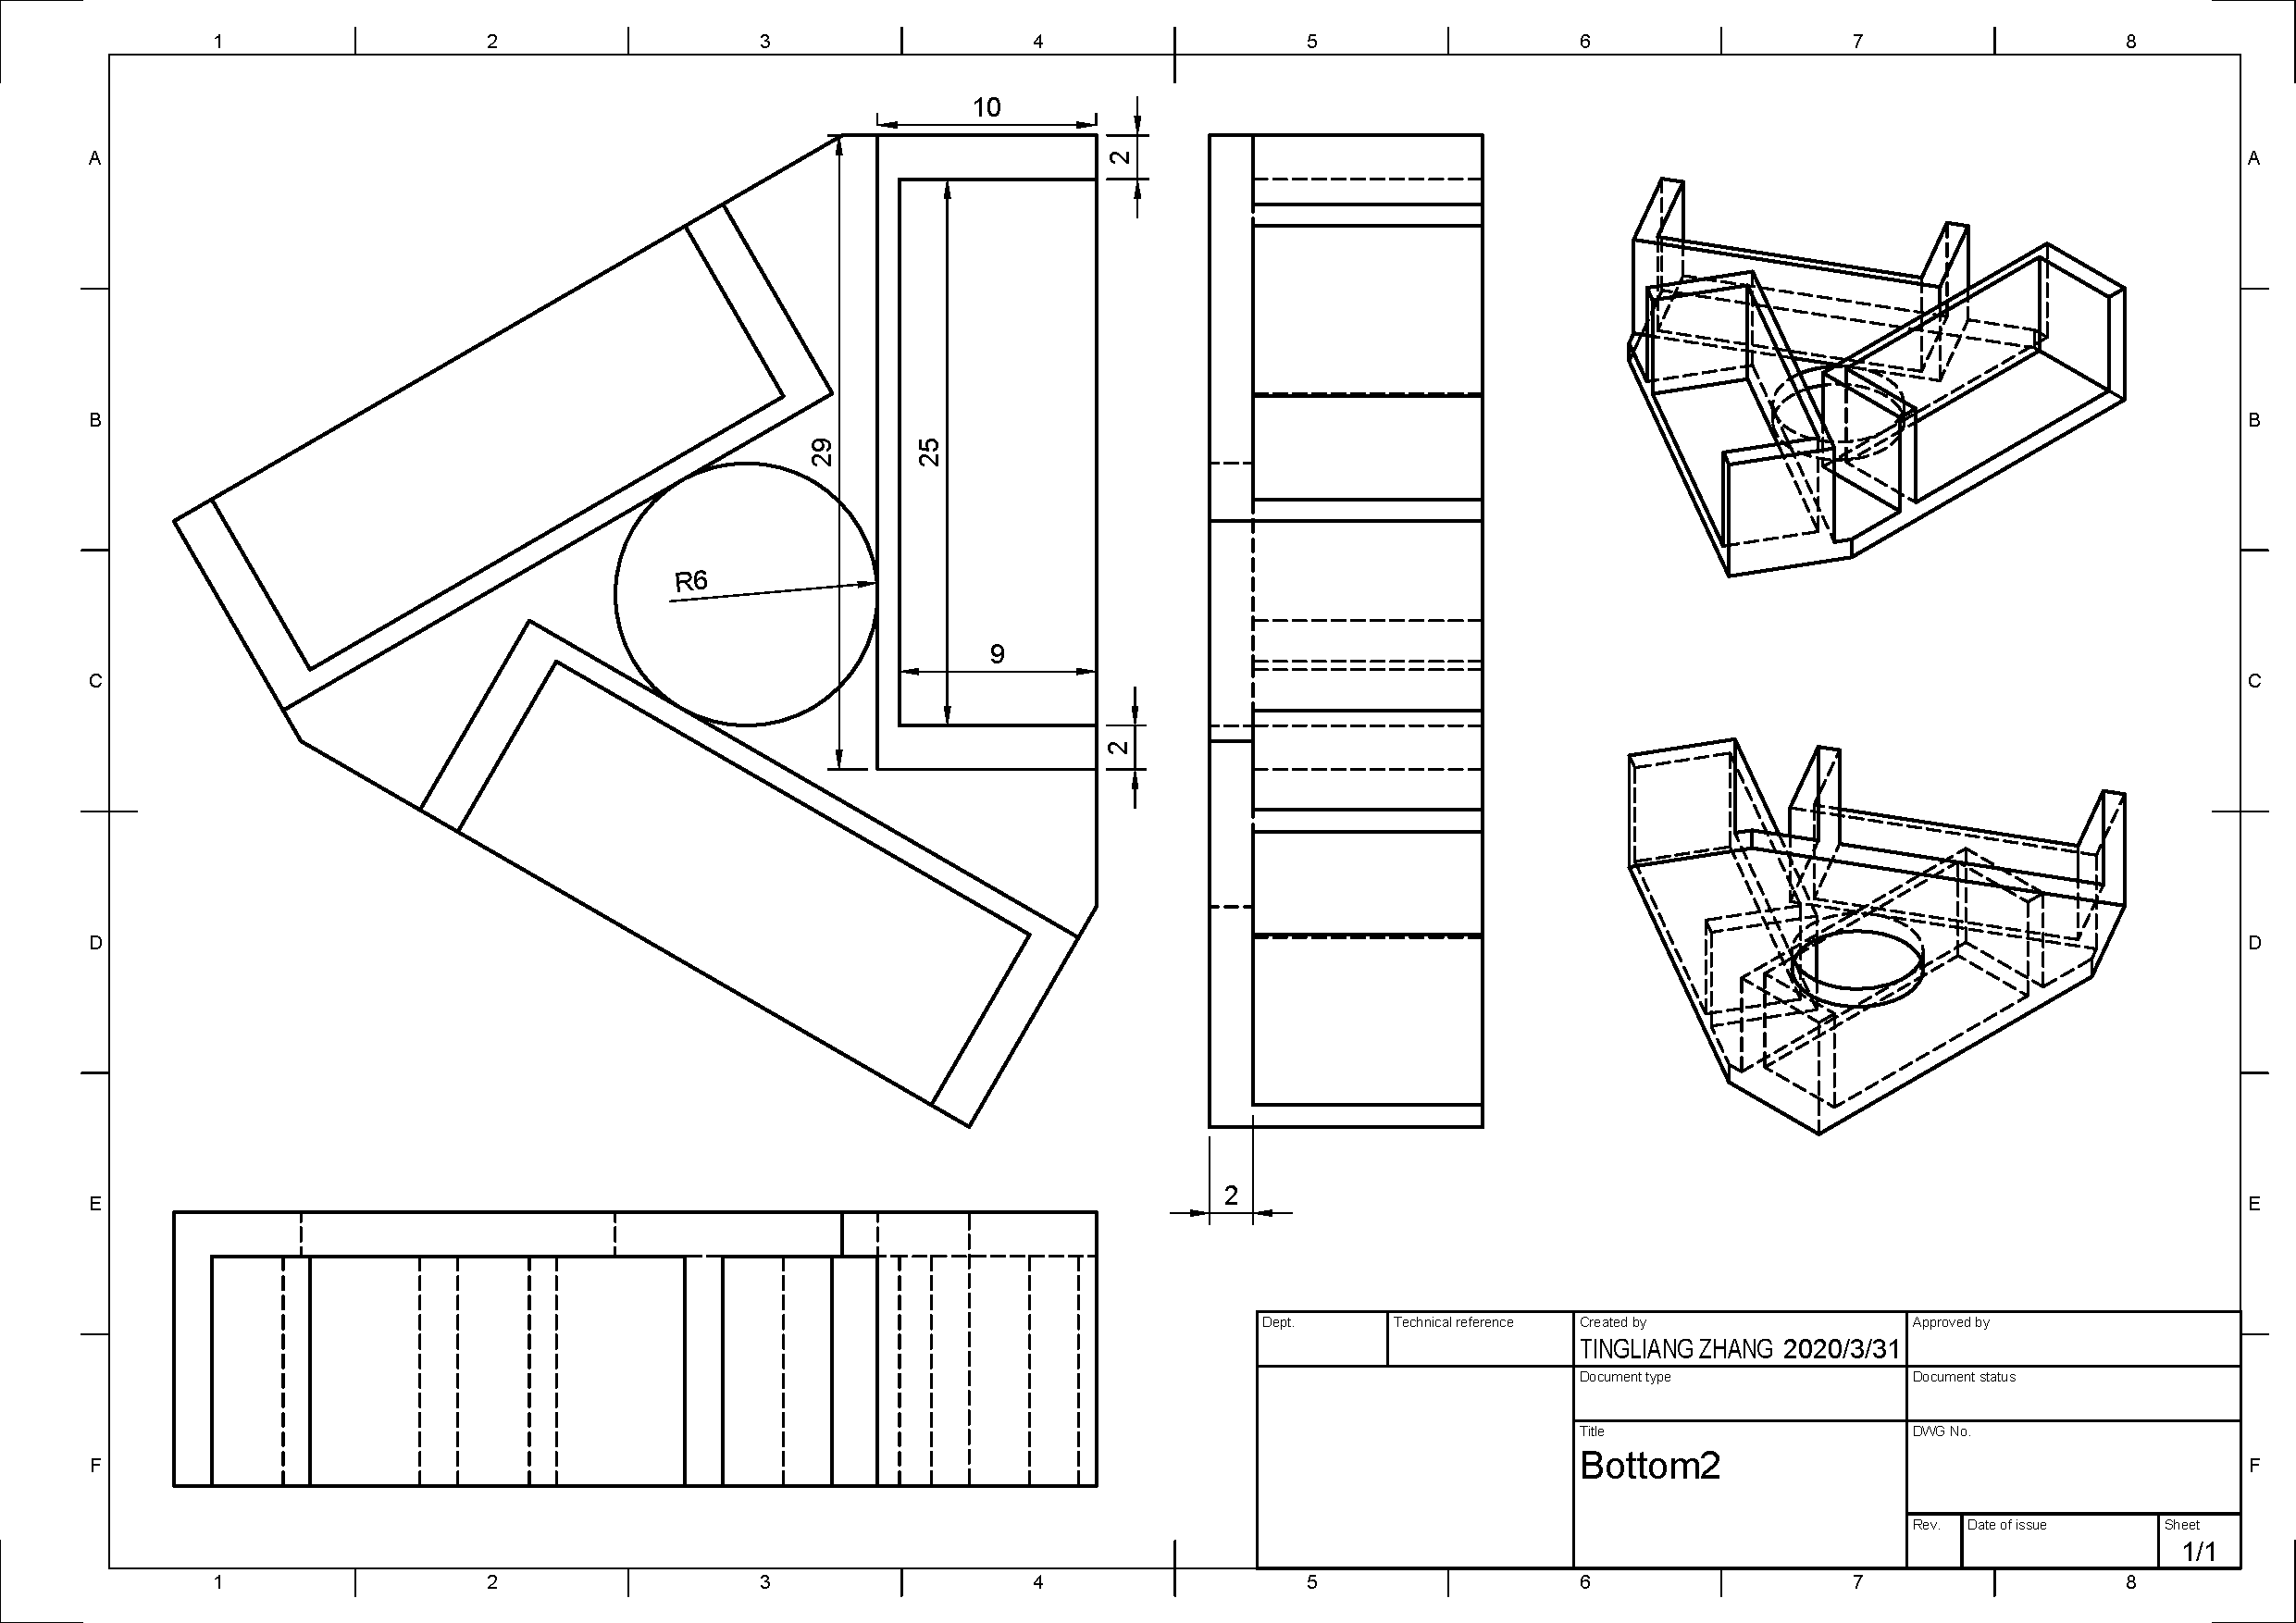
\includegraphics[width=\columnwidth]{Bottom2v1.pdf}
    \caption{v2测试底座图纸}
    \label{fig:Bottom2v1}
\end{figure}

\section{Model v3}

图纸如图~\ref{fig:BottomMountTest2}和图~\ref{fig:Bottom5v2}。

\begin{figure}[htbp]
    \centering
    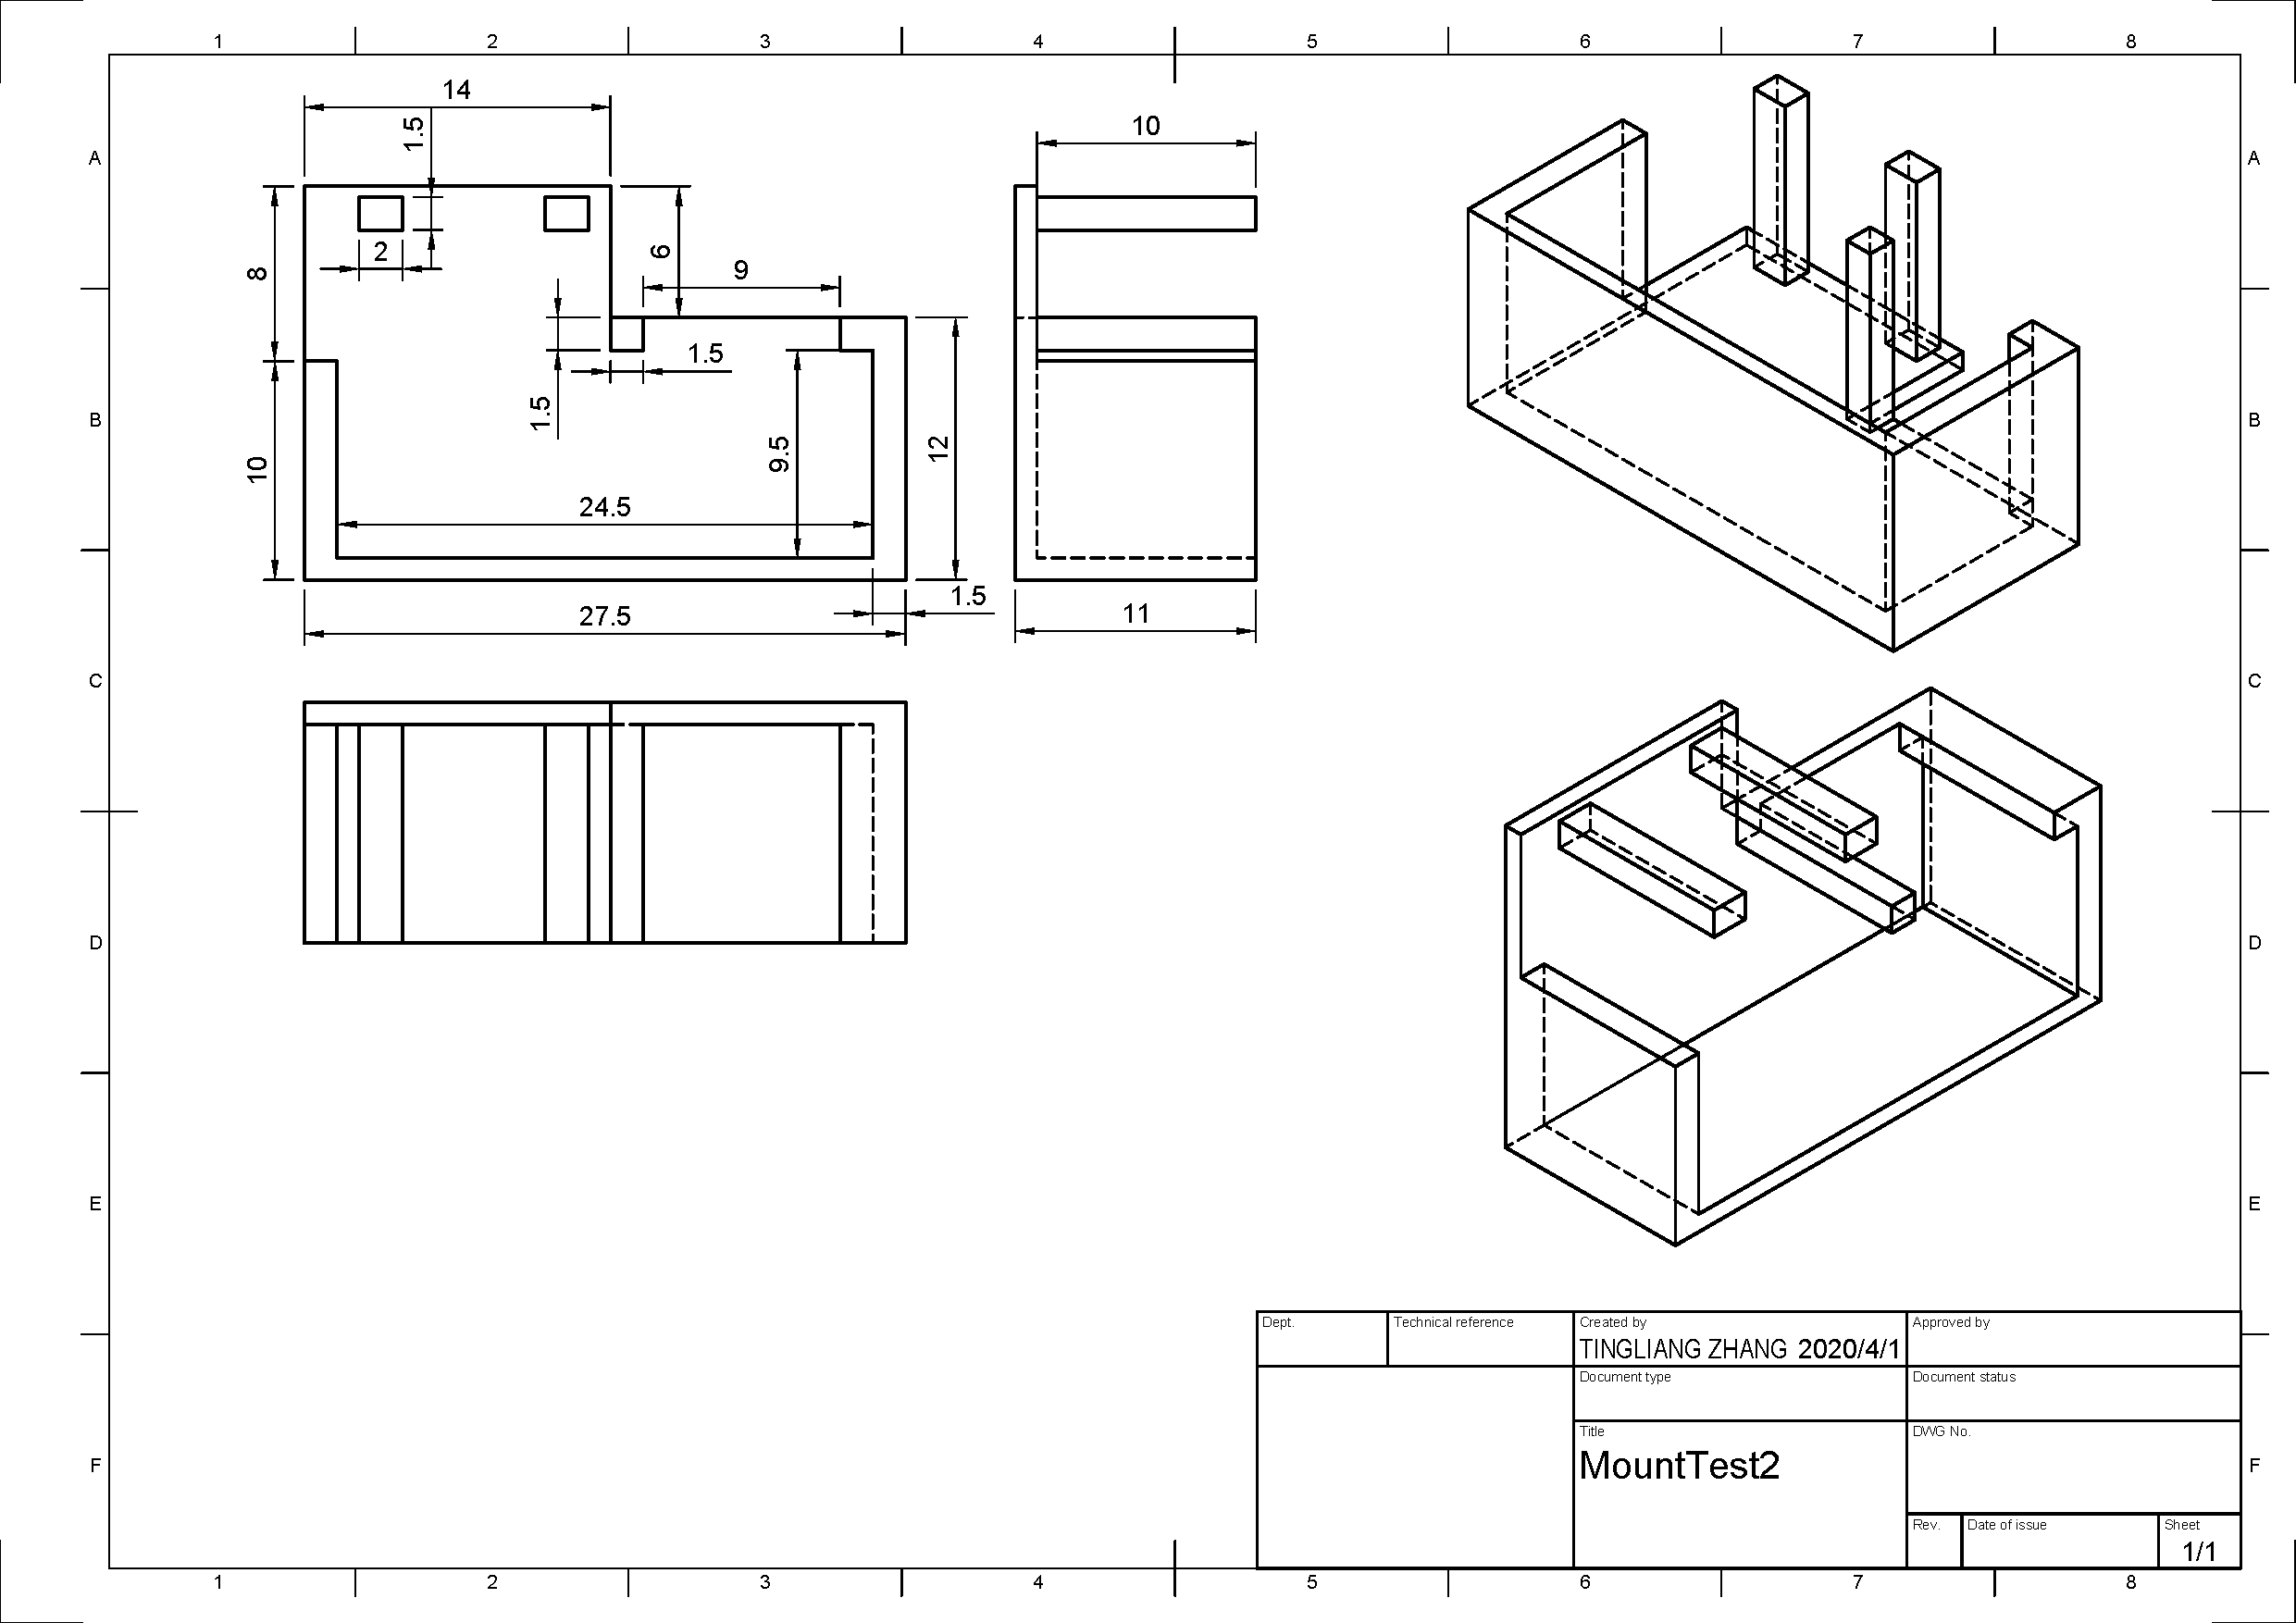
\includegraphics[width=\columnwidth]{BottomMountTest2.pdf}
    \caption{v3测试底座电机固定图纸}
    \label{fig:BottomMountTest2}
\end{figure}

图纸如图~\ref{fig:Bottom2v1}。

\begin{figure}[htbp]
    \centering
    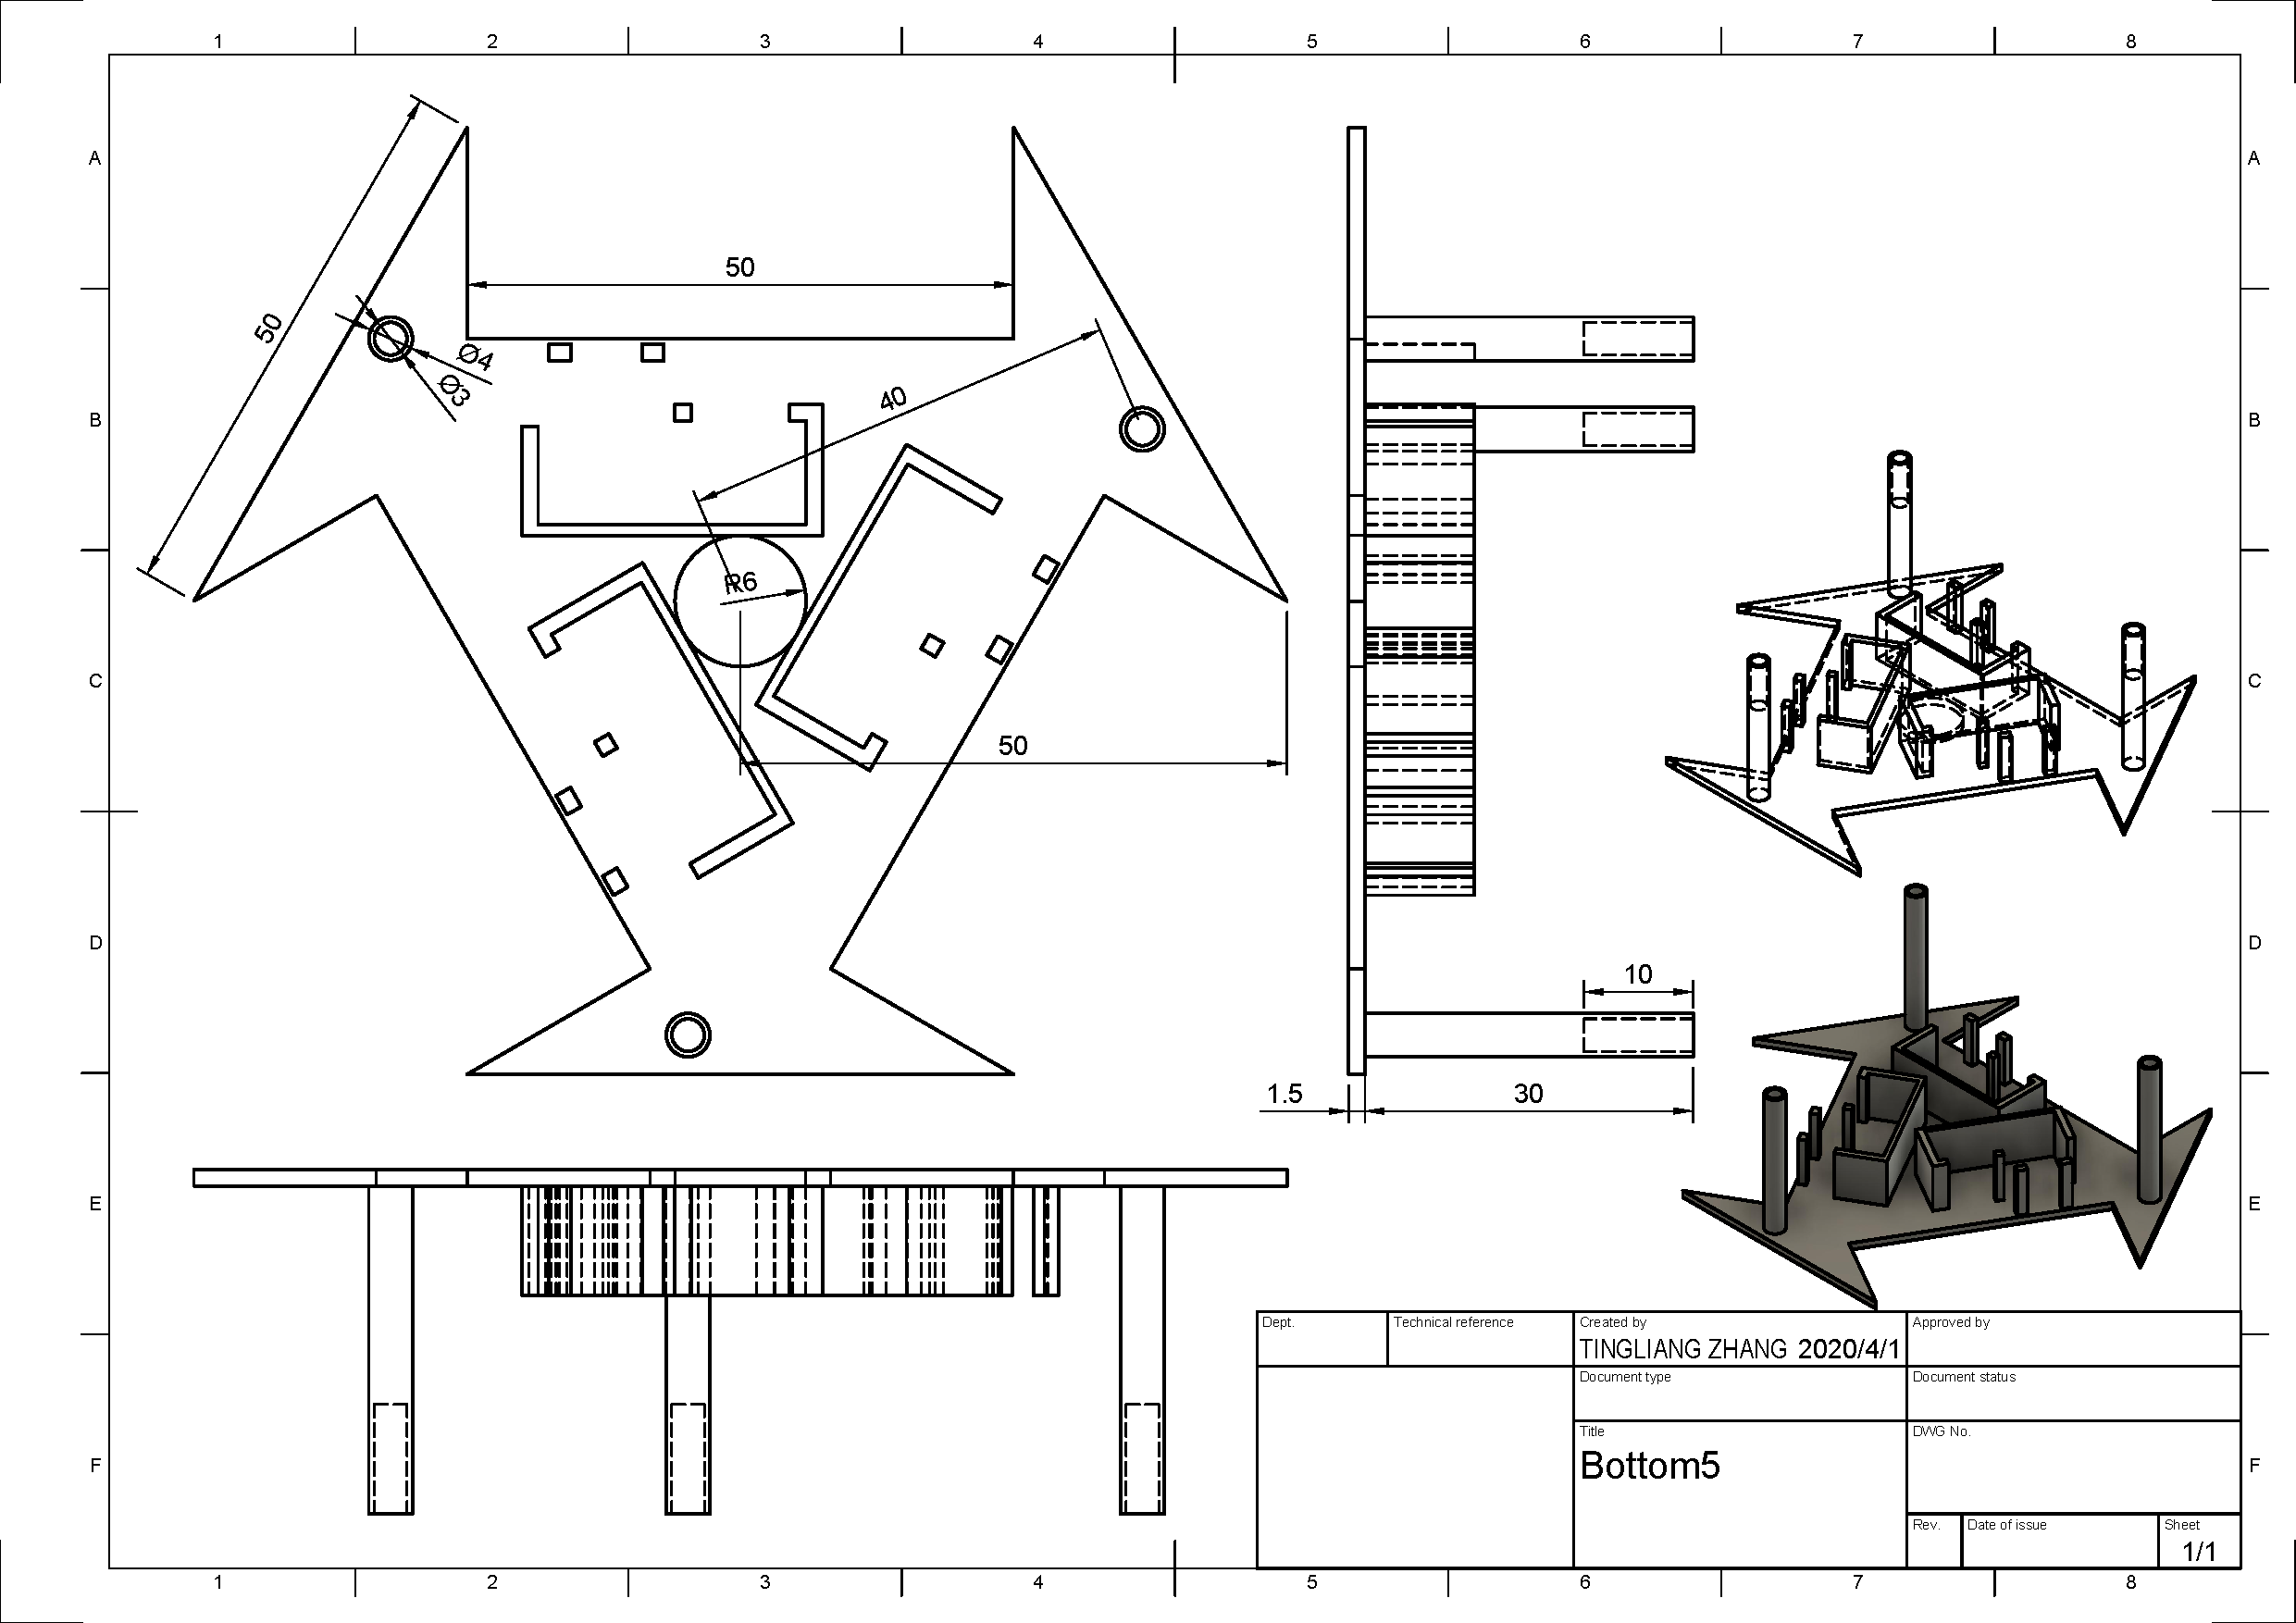
\includegraphics[width=\columnwidth]{Bottom5v2.pdf}
    \caption{v3测试底座整体图纸}
    \label{fig:Bottom5v2}
\end{figure}

v3底盘打印效果如图~\ref{fig:Bottom5}。

\begin{figure}[htbp]
    \centering
    \includegraphics[width=\columnwidth]{Bottom5.jpg}
    \caption{v3底盘打印效果}
    \label{fig:Bottom5}
\end{figure}

实物装配图如图~\ref{fig:Bottom-v3}。

\begin{figure}[htbp]
    \centering
    \includegraphics[width=\columnwidth]{Bottom-v3.jpg}
    \caption{v3底盘实物装配图}
    \label{fig:Bottom-v3}
\end{figure}

经过几十次反复打样测试,误差做到了0.1mm级别,不需要热熔胶就能靠摩擦力牢牢卡在正确的位置,当然如果想要更高的可靠性,可以在两侧加上两小滴热熔胶。

\section{Model v4}

测试过程中,发现电机固定联轴器的m3x8螺丝在转动过程中会碰到底盘。所以挖一个孔使其不会碰到底盘。

\section{3D打印}

使用极光尔沃 A3S 3D打印机(如图~\ref{fig:A3S})进行打样。详细参数如表~\ref{tab:A3S}。

\begin{figure}[htbp]
    \centering
    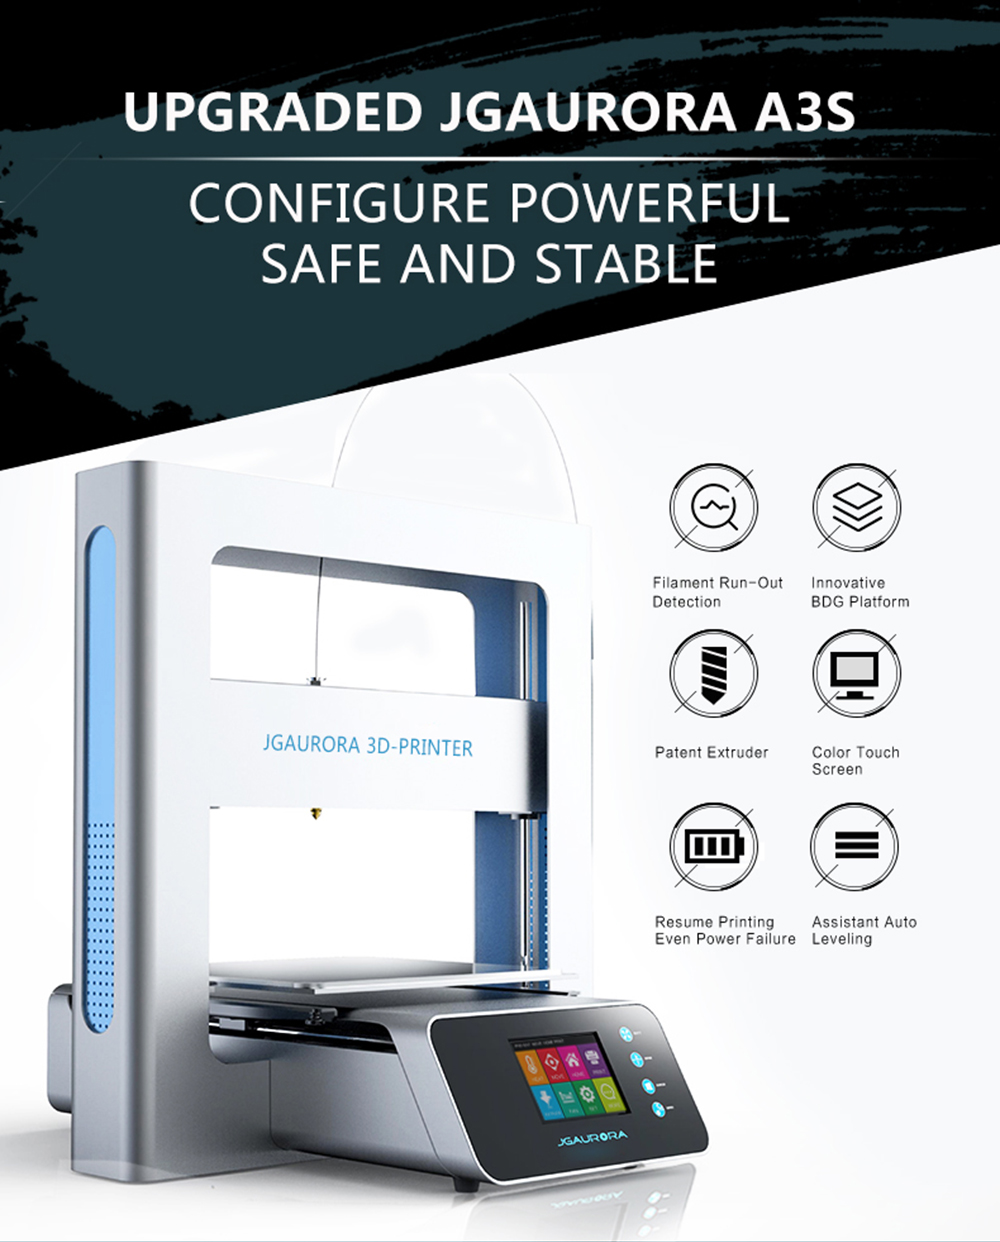
\includegraphics[width=0.6\columnwidth]{JGAurora-A3S.jpg}
    \caption{JGAurora A3S}
    \label{fig:A3S}
\end{figure}

\begin{table}[htbp]
    \centering
    \begin{tabular}{ll}
    Nozzle No.                  & Single                              \\
    Layer thickness             & 0.1-0.3mm                           \\
    Filament Diameter           & 1.75mm                              \\
    Build Size                  & 205*205*205mm                       \\
    Printing Accuracy           & 0.2mm                               \\
    Printing Speed              & 10-150 mm/s (Suggest 80mm/s)        \\
    Nozzle Diameter             & 0.4mm                               \\
    Nozzle Temp.                & 180$\sim$240℃                       \\
    Hot bed Temp.               & Room Temp.$\sim$110℃                \\
    Machine Size                & 431(Length)*370(Width)*423(Height)  \\
    Machine Weight              & 9kg                                 \\
    Packing Size                & 505(Length)*430(Width)*245(Height)  \\
    Packing Weight              & 11.5kg                              \\
    Power                       & 180W                                \\
    Leveling                    & Manual                              \\
    Control Panel               & 2.8 HD Touch LCD Display            \\
    Display Language            & English/Chinese                     \\
    Compatible Filament         & PLA/ABS/Wood/TPU, ect               \\
    Supported File              & STL、OBJ、G-Code                      \\
    Hot Bed                     & Black Diamond Glass Heated platform \\
    Pause Printing              & Support                             \\
    Power Failure Protection    & Support                             \\
    Filament Shortage Detection & Support                             \\
    U Stick Connection          & Support                             \\
    Slice Software              & Cura/Simplify3D/Slic3r/JGcreat     
    \end{tabular}
    \caption{JGAurora A3S Technical Specifications}
    \label{tab:A3S}
\end{table}

\subsection{Debug}

由于A3S是一款轻量级桌面打印机,并非商用级别,所以存在很多问题,下面对打印过程中遇到的问题进行阐述。

在初次组装完成或移动打印机之后需要重新调平,在平面上五点使用调平卡片进行调平。打印的时候喷头曾多次将打印件带起来,也就是打印件粘不住平台,可能是因为喷头和平台距离远,第一层压得不够瘪,耗材粘的不牢固,需要重新调平,另外切片时“打印平台附着类型”可以选择Brim/Raft来增大模型接触面。

PLA耗材曾多次断在料管里,需要按住端口的圈拔出白色料管,用新料疏通。

四月一日换料出现一次喷头不出料,疑似喷头堵料,拔下料管后,使用1.5号六角扳手怼进去疏通,用新料直接捅进喷头合适角度挤压出料后在用料管里面的料挤压,最后插上料管。

在维修打印机期间浪费了不少时间。

\subsection{切片软件}

使用开源的Ultimaker Cura 4.5作为切片软件,打印机配置选择JGAurora A3S即可导入打印机Config,耗材选Generic PLA,导入stl文件默认选项打印即可。

如图~\ref{fig:Cura}。

\begin{figure}[htbp]
    \centering
    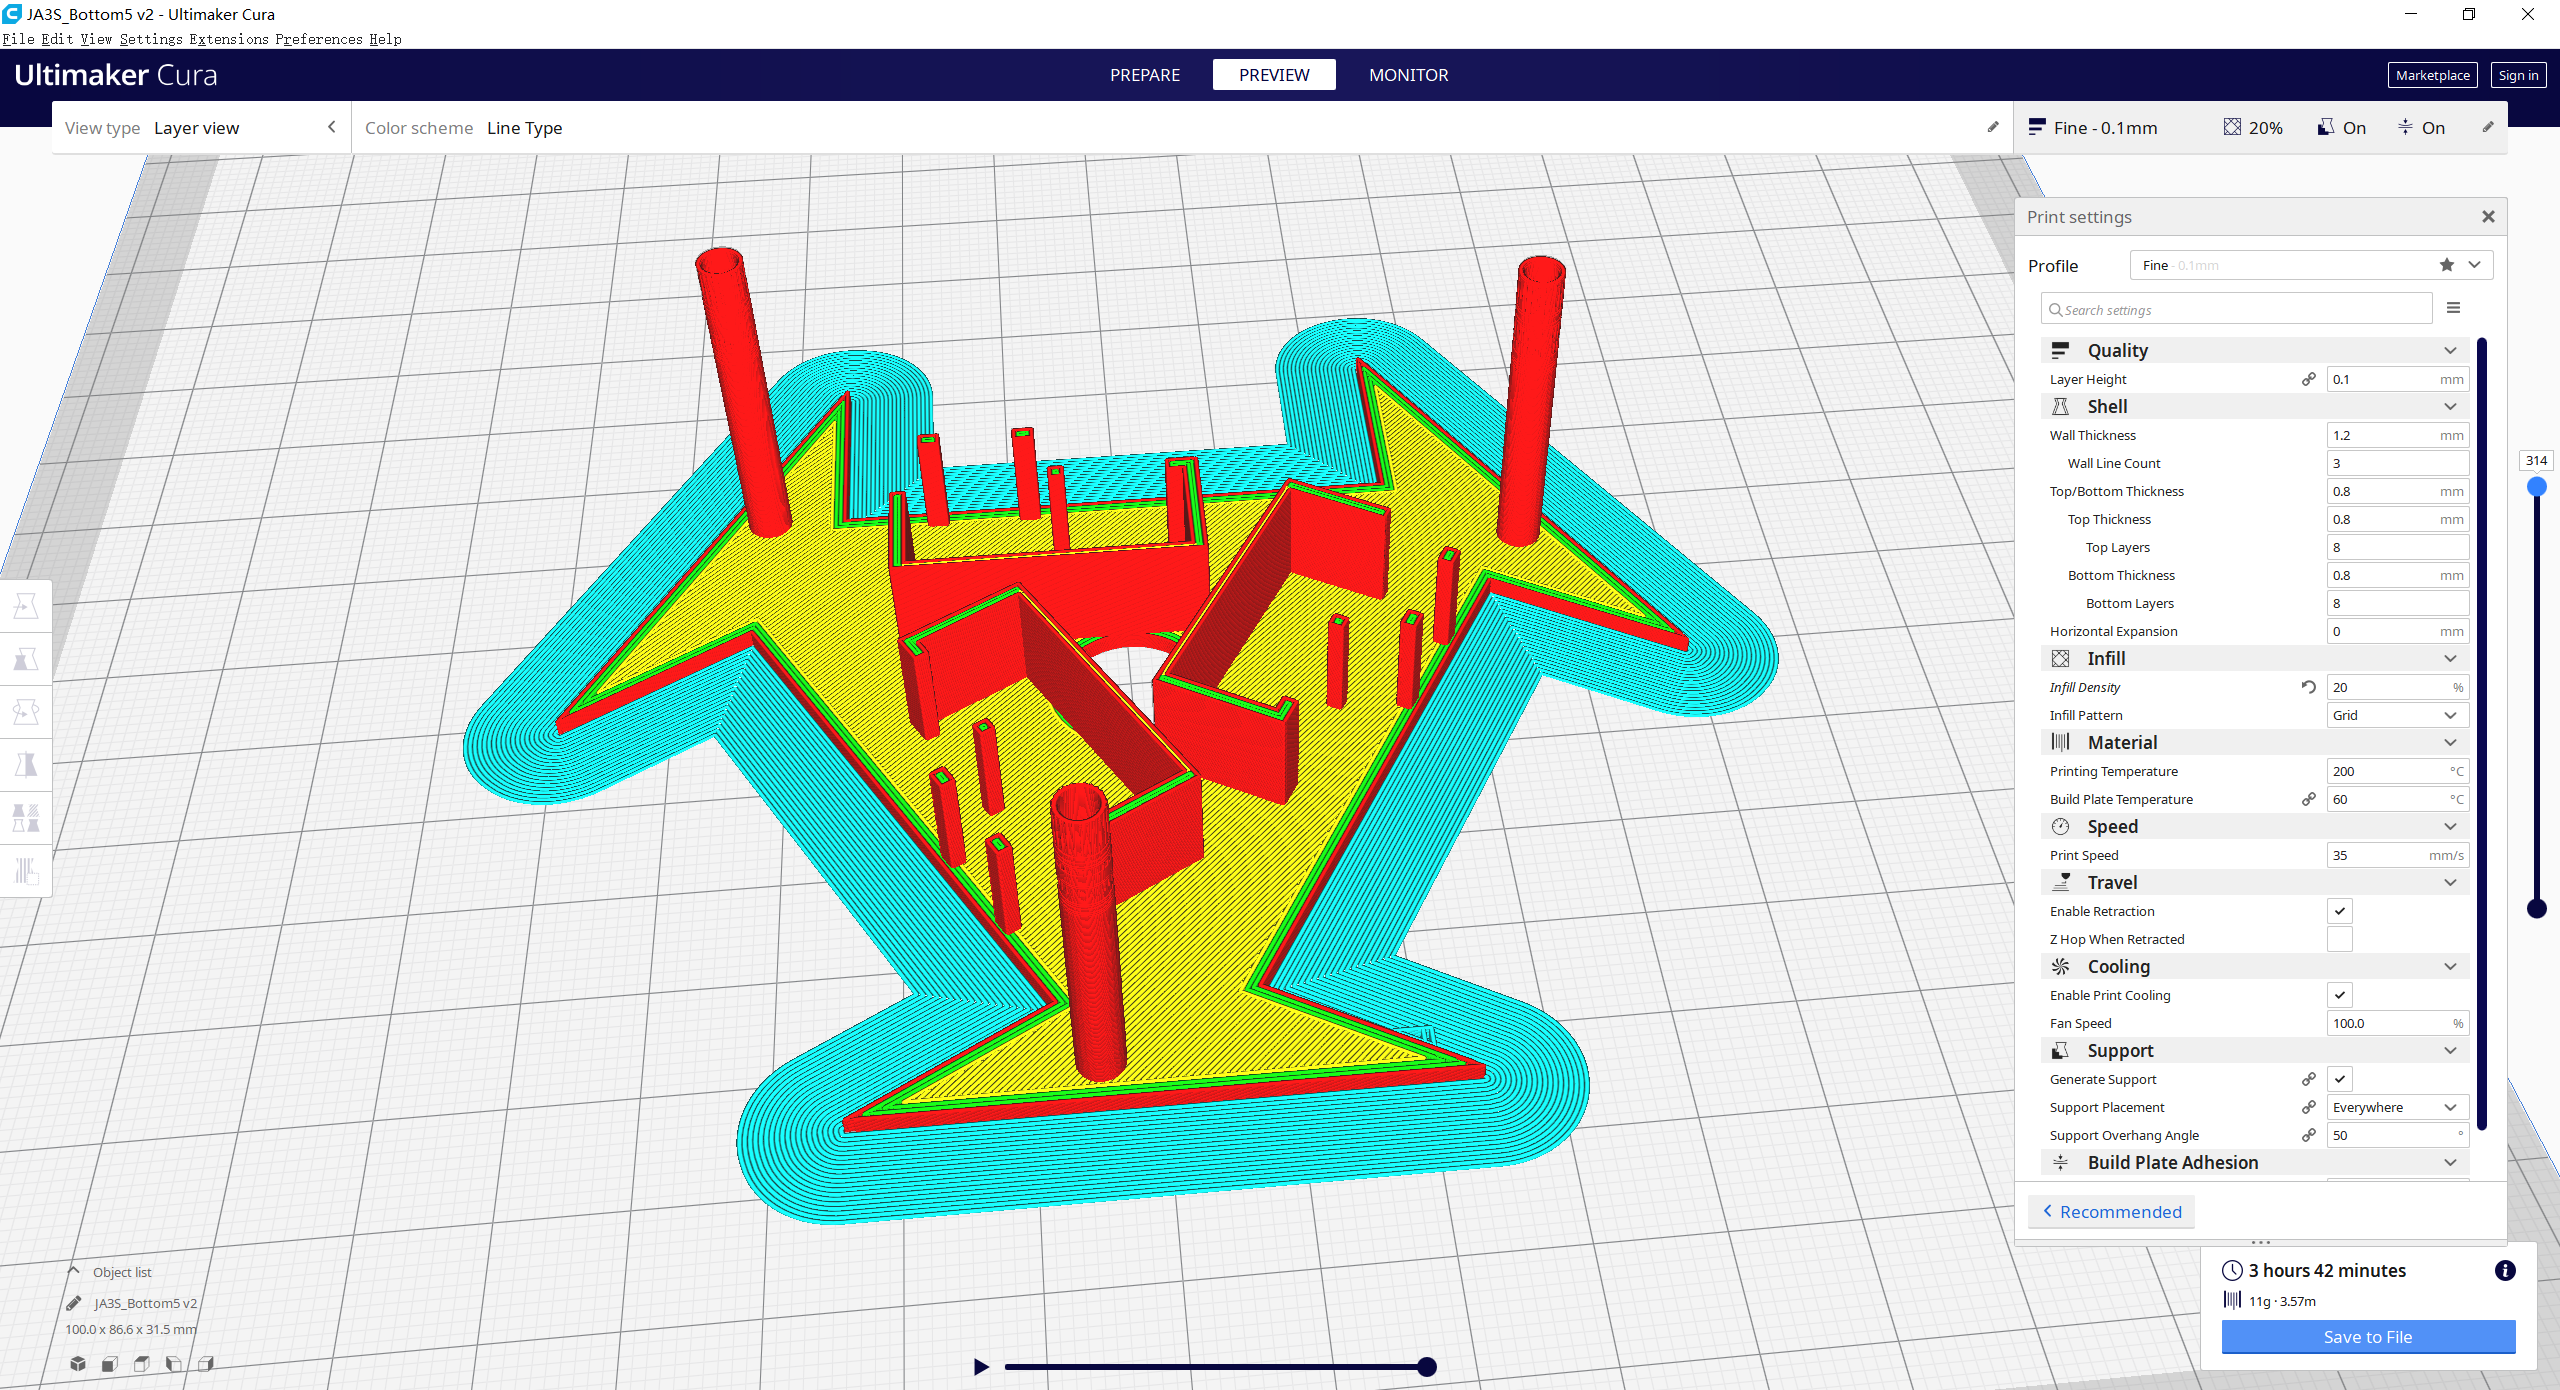
\includegraphics[width=\columnwidth]{Cura.png}
    \caption{Ultimaker Cura 4.5}
    \label{fig:Cura}
\end{figure}
